\section{Referencial Teórico e Estado da Arte}
\label{sec:referencial}

\subsection{Licitações Públicas}

A licitação pública constitui o procedimento administrativo formal por meio do qual a Administração Pública seleciona fornecedores para a aquisição de bens, prestação de serviços ou execução de obras, em atendimento ao disposto no art.~37, inciso XXI, da Constituição Federal e na Lei nº 14.133/2021~\cite{brasil2021licitacoes}. Seu objetivo central é assegurar a seleção da proposta apta a gerar o resultado mais vantajoso para o interesse público, garantindo igualdade de condições entre os concorrentes e publicidade dos atos praticados ao longo do certame.

Conforme ilustrado na Figura~\ref{fig:fluxograma_licitacao}, o rito licitatório origina-se a partir de uma necessidade identificada pela Administração Pública e desenvolve-se de forma sequencial em cinco etapas principais até a celebração da contratação:

\begin{enumerate}
  \item \textbf{Abertura e Edital:} compreende a definição do órgão demandante, do objeto a ser contratado e da modalidade licitatória aplicável, formalizada com a publicação do instrumento convocatório;
  \item \textbf{Itens e Cotação:} envolve o detalhamento e a especificação de lotes ou itens individuais, com suas respectivas quantidades, bem como a realização de pesquisa prévia para estabelecer os preços de referência;
  \item \textbf{Habilitação:} consiste na conferência documental da qualificação jurídica, regularidade fiscal, capacidade técnica e idoneidade econômica das empresas interessadas em disputar o certame;
  \item \textbf{Disputa e Julgamento:} corresponde à fase competitiva propriamente dita, marcada pelo envio de propostas e lances por item e pela subsequente classificação da melhor oferta segundo os critérios definidos no edital;
  \item \textbf{Homologação:} encerra formalmente o procedimento administrativo mediante a adjudicação do objeto ao proponente vencedor e a validação da regularidade do processo, viabilizando a etapa final de contratação.
\end{enumerate}

\begin{figure*}[!h]
  \centering
  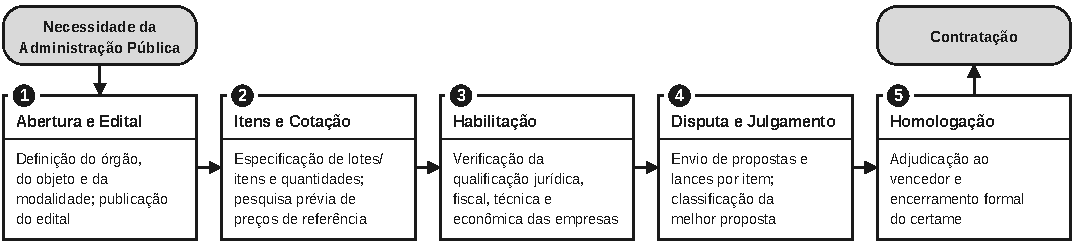
\includegraphics[width=0.95\textwidth]{figures/fluxograma_licitacao_horizontal.pdf}
  \caption{Fluxo sequencial das etapas do procedimento licitatório, desde a identificação da necessidade da Administração Pública até a efetivação da contratação, passando pelas fases de abertura e edital, especificação de itens e cotação, habilitação, disputa e julgamento, e homologação.}
  \label{fig:fluxograma_licitacao}
\end{figure*}

Sob a perspectiva da análise de dados e de redes, as fases de habilitação e de disputa e julgamento assumem papel central, pois registram formalmente quais empresas atuaram como competidoras simultâneas em um mesmo certame ou item. Quando examinadas de forma isolada por procedimento, as propostas podem aparentar competitividade regular; entretanto, a agregação desses registros ao longo de múltiplos certames permite observar padrões recorrentes de co-participação e investigar se agentes formalmente distintos compartilham vínculos societários ou cadastrais capazes de comprometer a independência efetiva da disputa.

\subsection{Fundamentos Jurídico-Regulatórios e Triagem Indiciária}

As contratações públicas devem assegurar tratamento isonômico entre os participantes e selecionar a proposta apta a produzir o resultado mais vantajoso para a Administração, conforme os princípios e objetivos estabelecidos pela Lei nº 14.133/2021~\cite{brasil2021licitacoes}. O diploma também prevê infrações administrativas relacionadas à fraude e à frustração do caráter competitivo dos procedimentos licitatórios. No plano concorrencial, a Lei nº 12.529/2011 considera infrações à ordem econômica condutas concertadas entre concorrentes que tenham por objeto ou possam produzir efeitos anticoncorrenciais~\cite{brasil2011concorrencia}. A Lei nº 12.846/2013, por sua vez, estabelece a responsabilização administrativa e civil de pessoas jurídicas pela prática de atos lesivos contra a Administração Pública, incluindo condutas relacionadas a procedimentos licitatórios~\cite{brasil2013anticorrupcao}.

Esse enquadramento jurídico justifica a adoção de mecanismos de prevenção e detecção de sinais de risco, mas não autoriza equiparar uma coincidência cadastral à comprovação de conluio. A existência de sócios em comum, endereços coincidentes, telefones compartilhados ou sobrenomes semelhantes pode constituir elemento para aprofundamento da análise, desde que interpretada em conjunto com o contexto da contratação e com outros elementos objetivos. A abordagem deste trabalho é, portanto, de triagem indiciária: os resultados destinam-se a apoiar a priorização de verificações, não a estabelecer responsabilidade administrativa ou penal.

A proteção de dados pessoais também deve ser considerada. A Lei nº 13.709/2018 (LGPD) disciplina o tratamento de dados pessoais de pessoas naturais e prevê disposições específicas para tratamentos realizados para fins acadêmicos, observadas as condições legais aplicáveis~\cite{brasil2018lgpd}. A pseudonimização reduz a exposição direta de identificadores, mas não equivale necessariamente à anonimização e não afasta, por si só, a incidência da legislação. Além disso, pessoas jurídicas não são titulares de dados pessoais para os fins da LGPD, embora a substituição de seus identificadores por rótulos possa ser adotada como medida de apresentação e governança dos dados. Neste estudo, os identificadores pessoais e empresariais são substituídos por códigos no material divulgado.

\subsection{Redes de Co-disputa, Relações Societárias e Homofilia}

A análise de riscos em licitações pode ser formulada como um problema relacional: além das características individuais dos fornecedores, interessam as relações estabelecidas entre empresas que participam dos mesmos procedimentos e entre essas empresas e seus sócios ou controladores. Guias da Organização para a Cooperação e Desenvolvimento Econômico (OCDE) e do Conselho Administrativo de Defesa Econômica (CADE) descrevem práticas colusivas como divisão de mercado, rodízio de vencedores, propostas de cobertura e supressão de propostas~\cite{oecd2025guidelines,cade2019guia}. Indicadores observáveis nos dados administrativos podem, assim, auxiliar a seleção de procedimentos que mereçam análise aprofundada~\cite{carbone2024bidrigging,fazekas2016objective,wachs2020corruption}.

Estudos sobre redes de co-participação demonstram que as relações entre fornecedores podem revelar padrões que não são evidentes quando cada procedimento é examinado isoladamente~\cite{wachs2019cartel,lyra2021characterization}. Pesquisas sobre propriedade e gestão também destacam a importância de considerar vínculos diretos e indiretos entre empresas concorrentes~\cite{villamil2024collusion,pompeu2025collusion}. Essas abordagens fundamentam a integração, neste trabalho, entre a camada de co-disputa e a camada de propriedade societária.

A interpretação de coincidências nominais exige cautela. O conceito de homofilia descreve a tendência de atores com características semelhantes estabelecerem relações entre si~\cite{mcpherson2001homophily}. Em dados cadastrais, sobrenomes frequentes podem ocorrer em empresas sem relação societária ou operacional. Por esse motivo, a coincidência de sobrenomes é tratada como atributo de menor força do que a identidade direta de sócios, endereço ou telefone. A ponderação discreta adotada neste trabalho é inspirada no princípio de reduzir a influência de atributos frequentes, mas não corresponde ao cálculo clássico de frequência inversa de documentos (IDF).

\subsection{Grafos Heterogêneos e Multicamadas}

Redes heterogêneas permitem representar entidades de diferentes tipos em uma mesma estrutura, enquanto modelos multicamada distinguem categorias de relações que coexistem entre essas entidades~\cite{kivela2014multilayer,newman2018networks}. Essa distinção é relevante para o problema estudado: órgãos públicos, empresas licitantes e integrantes do QSA (sócios, controladores e administradores) constituem tipos distintos de vértices; participação em licitação, co-disputa, vínculos societários/administrativos e vínculo suspeito constituem camadas relacionais distintas.

O grafo utilizado pode ser formalizado por
\begin{equation}
  G=(V,E,\tau_V,\tau_E,w),
  \label{eq:grafo_multicamada}
\end{equation}
em que $V$ é o conjunto de vértices, $E$ é o conjunto de arestas, $\tau_V:V\rightarrow\mathcal{T}_V$ associa cada vértice a um tipo, $\tau_E:E\rightarrow\mathcal{T}_E$ identifica a camada de cada aresta e $w:E\rightarrow\mathbb{R}_{>0}$ atribui pesos às relações.

Neste estudo, os tipos de vértices são órgãos públicos, empresas licitantes e integrantes do QSA (sócios, controladores e administradores). As quatro camadas de arestas são:
\begin{itemize}
  \item \texttt{Participou\_Licitacao}: conecta empresas aos órgãos responsáveis pelos certames dos quais participaram;
  \item \texttt{Concorreu\_Contra}: conecta pares de empresas que compartilharam participação no mesmo certame ou disputaram os mesmos itens, com peso associado à soma de certames e itens em comum;
  \item \texttt{É\_Dono\_De}: conecta integrantes do QSA (sócios, controladores ou administradores) e titulares de MEI às empresas às quais estão vinculados;
  \item \texttt{Vinculo\_Suspeito}: conecta empresas co-disputantes para as quais foi identificado escore positivo acima do limite mínimo de retenção.
\end{itemize}

As camadas \texttt{Participou\_Licitacao} e \texttt{É\_Dono\_De} são bipartidas entre tipos distintos de vértices. Já \texttt{Concorreu\_Contra} e \texttt{Vinculo\_Suspeito} conectam empresas entre si. Consequentemente, o grafo agregado não é, em geral, bipartido, ainda que algumas de suas camadas o sejam. Essa distinção é necessária para interpretar corretamente os motivos triangulares examinados neste trabalho.

\subsection{Motivos Triangulares e Vínculos Societários Compartilhados}

Um triângulo $K_3$ é um subgrafo com três vértices distintos e uma aresta entre cada par de vértices. No problema estudado, considera-se um motivo triangular tipado formado por duas relações da camada \texttt{É\_Dono\_De} e uma relação entre empresas concorrentes. Para um membro do QSA $s$ (sócio, controlador ou administrador) compartilhado pelas empresas $a$ e $b$, o motivo é
\begin{equation}
  \{(s,a),(s,b),(a,b)\},
  \label{eq:motivo_triangular}
\end{equation}
em que $(s,a)$ e $(s,b)$ pertencem à camada \texttt{É\_Dono\_De}, enquanto $(a,b)$ pertence à camada \texttt{Vinculo\_Suspeito}.

O triângulo, portanto, não está presente na camada bipartida do QSA considerada isoladamente. Ele aparece na representação agregada que combina as duas relações societárias ou administrativas com a aresta entre as empresas. Se duas empresas concorrentes compartilham dois integrantes distintos no QSA, cada elemento da interseção desses conjuntos forma um motivo triangular. A existência desses motivos caracteriza uma sobreposição de propriedade ou de administração observável, mas não comprova, por si só, coordenação ilícita ou ausência efetiva de independência decisória.

\subsection{Fundamentos dos Algoritmos de Redução Topológica}

A rede completa contém relações de natureza distinta e vértices com diferentes níveis de conectividade. Para concentrar a análise nas relações prioritárias, aplica-se um predicado de retenção às arestas e, em seguida, removem-se os vértices que não possuem incidência no subgrafo filtrado. Essa operação deve ser distinguida de um subgrafo induzido por conjunto de vértices: o procedimento implementado seleciona arestas por tipo e peso e preserva inicialmente o conjunto de vértices, inclusive os que se tornam isolados.

O $1$-core de um grafo é o maior subgrafo induzido em que todos os vértices possuem grau mínimo igual ou superior a um. Para $k=1$, sua obtenção equivale à remoção dos vértices isolados, isto é, aqueles cujo grau é zero. Como esses vértices não possuem arestas incidentes, sua remoção não provoca uma cascata de exclusões em outros vértices. A noção de $k$-core é utilizada na análise de coesão estrutural de redes~\cite{seidman1983network}. Quando a operação consiste apenas em remover vértices de grau zero, a descrição mais precisa é remoção de isolados para obtenção do $1$-core.

Após a filtragem, a identificação de componentes conexas separa os conjuntos de vértices que permanecem conectados por caminhos. A estrutura disjoint-set, também denominada Union-Find, mantém uma partição dinâmica dos vértices por meio de operações de busca e união. Com compressão de caminho e união por posto ou tamanho, o custo amortizado de uma sequência de operações é quase linear, podendo ser expresso por
\begin{equation}
  O\big((|V|+|E|)\alpha(|V|)\big),
  \label{eq:complexidade_union_find}
\end{equation}
em que $\alpha$ é a função inversa de Ackermann~\cite{tarjan1975efficiency}.

A enumeração dos motivos triangulares pode explorar a estrutura específica do problema. Para cada aresta suspeita $(a,b)$ entre empresas, comparam-se os conjuntos de sócios associados a cada empresa:
\begin{equation}
  \mathrm{Donos}(a)\cap\mathrm{Donos}(b).
  \label{eq:intersecao_donos}
\end{equation}
Cada sócio presente nessa interseção forma, com as duas empresas, um motivo triangular tipado. Com conjuntos previamente indexados, a operação pode ser implementada por interseção de conjuntos; seu custo depende dos tamanhos dos conjuntos comparados. Uma estimativa superior simplificada é $O(|E_s|d_{\max})$, em que $E_s$ é o conjunto de arestas suspeitas examinadas e $d_{\max}$ é o maior número de sócios associado a uma empresa, assumindo consultas de pertinência em tempo médio constante.

\subsection{Ponderação de Similaridade e Controle de Falsos Positivos}

O coeficiente de Jaccard é uma medida de similaridade entre conjuntos, definida por
\begin{equation}
  J(A,B)=\frac{|A\cap B|}{|A\cup B|}.
\end{equation}
Embora útil em diversas aplicações, a normalização pela união pode reduzir a expressão da quantidade absoluta de itens compartilhados quando os conjuntos comparados possuem tamanhos muito diferentes. Por essa razão, a metodologia preserva contagens absolutas de co-disputa como atributo de recorrência, sem incorporá-las diretamente ao escore cadastral e societário.

A frequência inversa de documentos (IDF) reduz a contribuição de termos frequentes em uma coleção. Uma formulação clássica é
\begin{equation}
  \mathrm{IDF}(t)=\log\left(\frac{N}{f(t)}\right),
\end{equation}
em que $N$ representa o número de documentos e $f(t)$ a quantidade de documentos que contêm o termo $t$. A implementação deste estudo não calcula essa expressão. Em seu lugar, utiliza uma ponderação discreta: sobrenomes previamente classificados como triviais recebem peso $0{,}25$, enquanto os demais recebem peso $1{,}00$. A regra é inspirada no princípio de reduzir a influência de atributos frequentes, mas deve ser caracterizada como heurística determinística, e não como aplicação integral de IDF.

\subsection{Síntese do Enquadramento e Limites Interpretativos}

O referencial sustenta a integração de relações licitatórias, societárias e cadastrais em um grafo heterogêneo multicamada. A literatura de redes fornece instrumentos para representar e examinar essas relações; os fundamentos algorítmicos justificam a filtragem e a redução estrutural; e o enquadramento jurídico delimita os resultados como sinais para triagem e priorização de auditorias. A metodologia não busca inferir automaticamente a ocorrência de conluio, mas identificar configurações relacionais que mereçam verificação documental e contextual pelos órgãos competentes.
